\documentclass[pra,12pt]{revtex4}
\usepackage{amsmath}
\usepackage{amssymb}
\usepackage{graphicx}
\usepackage{color}
\usepackage{mathrsfs}
\usepackage{enumerate}
\usepackage{epigraph}
\usepackage[pdfborder={0 0 0},colorlinks=true,linkcolor=blue,urlcolor=blue]{hyperref}

\def\ket#1{\left|#1\right\rangle}
\def\bra#1{\left\langle#1\right|}
\def\braket#1{\left\langle#1\right\rangle}

\setlength{\parindent}{0pt}

\renewcommand{\baselinestretch}{1.0}
\setlength{\parskip}{0.07in}
\setlength{\epigraphwidth}{.6\textwidth}

\begin{document}

\begin{center}
{\Large \textbf{Chapter 4: Quantum Electrodynamics}}
\end{center}

This chapter provides a survey of \textbf{quantum electrodynamics},
the quantum theory of the electromagnetic field and its interaction
with electrically charged particles, such as electrons.  We start by
formulating Hamiltonians to describe how a quantum mechanical electron
is affected by classical electric and magnetic fields.  Next, we
describe the quantization of Maxwell's equations, which yields a
quantum field theory in which the elementary excitations are
photons---particles of light.  The last step is to formulate a theory
in which both electrons and photons are treated on the same footing,
as excitations of underlying quantum fields.  Along the way, we will
see how relativity can be accomodated within quantum mechanics.

Quantum electrodynamics is a rich and intricate theory, and we will
not be able to cover a lot of important ground, such as the
relationship with special relativity and diagrammatic methods for
performing field theoretical calculations.  For further reading, the
interested student may refer to Dyson's 1951 lecture notes
(\hyperref[cite:dyson]{Dyson 1951}) and Zee's introductory textbook
\textit{Quantum Field Theory in a Nutshell} (\hyperref[cite:zee]{Zee
  2010}).

\section{Particles in a classical electromagnetic field}

\subsection{Non-relativistic spinless particles in an electromagnetic field}
\label{sec:nonrel}

Consider a non-relativistic charged particle in an electromagnetic
field.  As we are mainly interested in the physics of electrons
interacting with electromagnetic fields, we will henceforth take the
electric charge of the particle to be $-e$, where $e =
1.602\times10^{-19}\,\mathrm{C}$ is the elementary charge.  (To
describe particles with an arbitrary electric charge $q$, simply
perform the substitution $e \rightarrow -q$ in all formulas in the
rest of this chapter.)

We wish to formulate the Hamiltonian governing the quantum dynamics of
such a particle, subject to two simplifying assumptions: (i) the
particle has charge and mass but is otherwise ``featureless'' (i.e.,
unlike a real electron, it has no spin angular momentum, and no
magnetic dipole moment), and (ii) the electromagnetic field is treated
as a classical field (i.e., the electric and magnetic fields are
definite quantities).

Let us first derive the \textit{classical} equations of motion.  In
the classical regime, the action of an electromagnetic field on a
point charged particle is decribed by the Lorentz force law,
\begin{equation}
  \mathbf{F}(\mathrm{r},t) = -e\Big(\mathbf{E}(\mathrm{r},t)
  + \dot{\mathbf{r}}\times \mathbf{B}(\mathrm{r},t)\Big),
\end{equation}
where $\mathbf{r}$ and $\dot{\mathbf{r}}$ respectively denote the
position and velocity of the particle, $t$ is the time, and
$\mathbf{E}$ and $\mathbf{B}$ are the electric and magnetic fields.
If there are no other forces acting on the particle, then according to
Newton's second law, the equation of motion is
\begin{equation}
  m\ddot{\mathbf{r}} = -e\Big(\mathbf{E}(\mathrm{r},t)
  + \dot{\mathbf{r}} \times \mathbf{B}(\mathrm{r},t)\Big),
  \label{eom}
\end{equation}
where $m$ is the particle's mass.  To quantize this, we must convert
this equation of motion into the form of Hamilton's equations of
motion.

First, we introduce the electromagnetic scalar and vector potentials
$\Phi(\mathrm{r},t)$ and $\mathbf{A}(\mathrm{r},t)$, where
\begin{align}
  \mathbf{E}(\mathbf{r},t) &= - \nabla \Phi(\mathbf{r},t) - \frac{\partial\mathbf{A}}{\partial t} \\
  \mathbf{B}(\mathbf{r},t) &= \nabla \times \mathbf{A}(\mathbf{r},t).
  \label{Bfield}
\end{align}
We now postulate that the above equation of motion can be described by
the Lagrangian
\begin{equation}
  L(\mathbf{r},\dot{\mathbf{r}},t) = \frac{1}{2}m\dot{\mathbf{r}}^2
  + e \Big[\Phi(\mathbf{r},t) - \dot{\mathbf{r}} \cdot \mathbf{A}(\mathbf{r},t)
    \Big].
\end{equation}
This is very similar to the usual prescription for the Lagrangian as
the kinetic energy minus the potential energy, with $-e\Phi$ serving
as the potential energy function.  However, there is an extra
$-e\dot{\mathbf{r}} \cdot \mathbf{A}$ term; this will turn out to be
responsible for the magnetic force.  Let us plug the Lagrangian into
the Euler-Lagrange equations:
\begin{equation}
  \frac{\partial L}{\partial r_i} = \frac{d}{dt}
  \frac{\partial L}{\partial \dot{r}_i}.
\end{equation}
The partial derivatives of the Lagrangian are:
\begin{align}
  \begin{aligned}
    \frac{\partial L}{\partial r_i} &=
    e\Big[\partial_i \Phi - \dot{r}_j \,\partial_i A_j \Big]\\
    \frac{\partial L}{\partial \dot{r}_i} &= m\dot{r}_i - e A_i.
  \end{aligned}
\end{align}
Now we want to take the \textit{total} time derivative of $\partial L
/\partial \dot{r}_i$.  In doing so, note that the $\mathbf{A}$ field
has its own $t$-dependence, as well as varying with the particle's
$t$-dependent position.  Thus,
\begin{align}
  \begin{aligned}
    \frac{d}{dt} \frac{\partial L}{\partial \dot{r}_i}
    &= m\ddot{r}_i - e\, \frac{d}{dt} A_i(\mathbf{r}(t),t) \\
    &= m\ddot{r}_i - e\, \partial_t A_i
    - e\, \dot{r}_j \partial_j A_i.
  \end{aligned}
\end{align}
(In the above equations, $\partial_i \equiv \partial/\partial r_i$,
where $r_i$ is the $i$-th component of the position vector, while
$\partial_t \equiv \partial/\partial t$.)  Plugging these expressions
into the Euler-Lagrange equations yields
\begin{align}
  \begin{aligned}
    m\ddot{r}_i &=
    -e\Big[\Big(-\partial_i \Phi - \partial_t A_i\Big)
      + \dot{r}_j \Big( \partial_i A_j - \partial_j A_i\Big) \Big] \\
    &= -e \Big[E_i(\mathbf{r},t) + \big(\dot{\mathbf{r}} \times
      \mathbf{B}(\mathbf{r},t) \big)_i\, \Big].
  \end{aligned}
\end{align}
(The last step can be derived by expressing the cross product using
the Levi-Cevita symbol, and using the identity $\varepsilon_{ijk}
\varepsilon_{lmk} = \delta_{il} \delta_{jm} - \delta_{im}
\delta_{jl}$.)  As desired, this is the equation of motion
corresponding to the Lorentz force.

We can now use the Lagrangian to derive the Hamiltonian.  The
canonical momentum is
\begin{equation}
  p_i = \frac{\partial L}{\partial \dot{r}_i} = m\dot{r}_i - e A_i.
\end{equation}
The Hamiltonian can be defined as $H(\mathbf{r},\mathbf{p}) =
\mathbf{p} \cdot \dot{\mathbf{r}} - L$.  This has to be expressed
using the $\mathbf{p}$ variables rather than $\dot{\mathbf{r}}$
variables:
\begin{align}
  \begin{aligned}
    H &= \mathbf{p}\cdot \left(\frac{\mathbf{p}+e\mathbf{A}}{m}\right)
    - \left(\frac{|\mathbf{p}+e\mathbf{A}|^2}{2m}
    + e\Phi - \frac{e}{m}(\mathbf{p}+e\mathbf{A})\cdot \mathbf{A}\right) \\
    &= \frac{|\mathbf{p}+e\mathbf{A}|^2}{m}
    - \frac{e}{m}\mathbf{A}\cdot \left(\mathbf{p}+e\mathbf{A}\right)
    - \left(\frac{|\mathbf{p}+e\mathbf{A}|^2}{2m}
    + e\Phi - \frac{e}{m}(\mathbf{p}+e\mathbf{A})\cdot \mathbf{A}\right).
  \end{aligned}
\end{align}
After cancelling various terms, we arrive at the result
\begin{equation}
H = \frac{|\mathbf{p}+e\mathbf{A}(\mathbf{r},t)|^2}{2m} - e\Phi(\mathbf{r},t).
\end{equation}

This looks a lot like the familiar Hamiltonian for a non-relativistic
particle that we have dealt with many times,
\begin{equation}
  H = \frac{|\mathbf{p}|^2}{2m} + V(\mathbf{r},t).
\end{equation}
The scalar potential $\Phi(\mathbf{r},t)$ enters into the potential
energy term, as might be expected.  What may be more surprising is
that the vector potential appears via the substitution
\begin{equation}
  \mathbf{p} \rightarrow \mathbf{p} + e\mathbf{A}(\mathbf{r},t).  
\end{equation}
What does this mean?

To answer this, think about what ``momentum'' means in the context of
a charged particle in an electromagnetic field.  The meaning of
``momentum'' is rooted in Noether's theorem, which states that every
symmetry of a system (whether classical or quantum) is associated with
a conserved quantity.  Momentum is the quantity conserved when the
system is symmetric under spatial translations.  We can see this from
the Hamilton equation
\begin{equation*}
  \frac{dp_i}{dt} = \frac{\partial H}{\partial r_i},
\end{equation*}
which implies that if a Hamiltonian is $\mathbf{r}$-independent, then
$d\mathbf{p}/dt = 0$.  But when the electromagnetic potentials are
$\mathbf{r}$-independent, the quantity $m\dot{\mathbf{r}}$ (which we
usually call momentum) is \textit{not} necessarily conserved!
Consider the potentials
\begin{equation}
  \Phi(\mathbf{r}, t) = 0, \;\;\; \mathbf{A}(\mathbf{r}, t) = Ct \hat{z},
\end{equation}
where $C$ is some constant.  These potentials are evidently
$\mathbf{r}$-independent, but the vector potential is time-dependent,
so the $-\dot{\mathbf{A}}$ term in Eq.~\eqref{Bfield} gives a
non-vanishing electric field:
\begin{equation}
  \mathbf{E}(\mathbf{r},t) = - C\hat{z}, \;\;\;\mathbf{B}(\mathbf{r},t) = 0.
\end{equation}
The Lorentz force law then says that
\begin{equation}
  \frac{d}{dt}(m\dot{\mathbf{r}}) = eC\hat{z},
\end{equation}
and thus $m\dot{\mathbf{r}}$ is not conserved.  On the other hand, the
quantity $\mathbf{p} = m\dot{\mathbf{r}} - e \mathbf{A}$ \textit{is}
conserved:
\begin{equation}
  \frac{d}{dt}(m\dot{\mathbf{r}} - e\mathbf{A}) =
  eC\hat{z} - eC\hat{z} = 0.
\end{equation}

The last step is to go from classical to quantum mechanics.  For this,
we merely need to replace $\mathbf{r}$ with the position operator
$\hat{\mathbf{r}}$, and $\mathbf{p}$ with the momentum operator
$\hat{\mathbf{p}}$.  Hence, the quantum Hamiltonian is
\begin{equation}
\boxed{\qquad
  \hat{H}(t) = \frac{|\hat{\mathbf{p}}+e\mathbf{A}(\hat{\mathbf{r}},t)|^2}{2m}
  - e\Phi(\hat{\mathbf{r}},t).\qquad}
  \label{quantumH}
\end{equation}
In the wavefunction representation, the momentum operator is
$\hat{\mathbf{p}} = -i\hbar\nabla$, as usual.

\subsection{Gauge symmetry}
\label{sec:gauge}

The Hamiltonian \eqref{quantumH} possesses a subtle property known as
\textbf{gauge symmetry}.  Suppose we modify the scalar and vector
potentials via the substitutions
\begin{align}
  \begin{aligned}
    \Phi(\mathbf{r},t) &\rightarrow \Phi(\mathbf{r},t) + \dot{\lambda}(\mathbf{r},t)\\
    \mathbf{A}(\mathbf{r},t) &\rightarrow
    \mathbf{A}(\mathbf{r},t) - \nabla{\lambda}(\mathbf{r},t),
  \end{aligned}
\end{align}
where $\lambda(\mathbf{r},t)$ is an arbitrary scalar field called a
\textbf{gauge field}.  This is the \textbf{gauge transformation} of
classical electromagnetism, which as we know leaves the electric and
magnetic fields unchanged.  When applied to the Hamiltonian
\eqref{quantumH}, it generates a new Hamiltonian,
\begin{equation}
  \hat{H}_\lambda(t)
  = \frac{|\hat{\mathbf{p}}+e\mathbf{A}(\hat{\mathbf{r}},t) + e\nabla\lambda(\hat{\mathbf{r}},t)|^2}{2m}
  - e\Phi(\hat{\mathbf{r}},t) - e\dot{\lambda}(\hat{\mathbf{r}},t).
\end{equation}
If $\psi(\mathbf{r},t)$ is any wavefunction obeying the Schr\"odinger
equation for the original Hamiltonian,
\begin{equation}
  i\hbar\frac{\partial\psi}{\partial t} =
  \hat{H}(t) \psi(\mathbf{r},t)
  = \left[\frac{|\hat{\mathbf{p}}+e\mathbf{A}(\hat{\mathbf{r}},t)|^2}{2m}
  - e\Phi(\hat{\mathbf{r}},t) \right]\psi(\mathbf{r},t),
\end{equation}
then it can be shown that the wavefunction $\psi(\mathbf{r},t)
\exp(ie\lambda/\hbar)$ automatically satisfies the Schr\"odinger
equation for the transformed Hamiltonian:
\begin{equation}
  i\hbar\frac{\partial}{\partial t} \left[\psi(\mathbf{r},t) \, \exp\left(\frac{ie\lambda(\mathbf{r},t)}{\hbar}\right)\right] =
  \hat{H}_\lambda(t) \left[\psi(\mathbf{r},t) \, \exp\left(\frac{ie\lambda(\mathbf{r},t)}{\hbar}\right)\right].
  \label{gaugeschrod}
\end{equation}

To prove this, observe how time and space derivatives act on the new
wavefunction:
\begin{align}
  \begin{aligned}
    \frac{\partial}{\partial t} \left[\psi \, \exp\left(\frac{ie\lambda}{\hbar}\right)\right] &=
    \left[\frac{\partial\psi}{\partial t} \;+\; \frac{ie}{\hbar} \dot{\lambda} \psi
      \,\, \right] \exp\left(\frac{ie\lambda}{\hbar}\right)\\
    \nabla \left[\psi \, \exp\left(\frac{ie\lambda}{\hbar}\right)\right] &=
    \left[\nabla \psi + \frac{ie}{\hbar} \nabla \lambda \psi \right] \exp\left(\frac{ie\lambda}{\hbar}\right).
  \end{aligned}
\end{align}
When the extra terms generated by the $\exp(ie\lambda/\hbar)$ factor
are slotted into the Schr\"odinger equation, they cancel the gauge
terms in the scalar and vector potentials.  For example:
\begin{align}
  \begin{aligned}
    \Big(-i\hbar\nabla + e\mathbf{A} - e\nabla\lambda\Big)
    \left[\psi \, \exp\left(\frac{ie\lambda}{\hbar}\right)\right] &=
    \Big[\left(-i\hbar\nabla + e\mathbf{A}\right)\psi\Big]\;
    \exp\left(\frac{ie\lambda}{\hbar}\right) \\
    \Big|-i\hbar\nabla + e\mathbf{A} - e\nabla\lambda\;\Big|^2
    \left[\psi \, \exp\left(\frac{ie\lambda}{\hbar}\right)\right] &=
    \Big[\left|-i\hbar\nabla + e\mathbf{A}\right|^2\psi\Big]\;
    \exp\left(\frac{ie\lambda}{\hbar}\right).
  \end{aligned}
\end{align}
The remainder of the proof for Eq.~\eqref{gaugeschrod} can be carried
out in a straightforward manner.


The above result can be stated in a simpler form if the
electromagnetic fields are static.  For static fields, the
time-independent electromagnetic Hamiltonian is
\begin{equation}
  \hat{H} = \frac{|\hat{\mathbf{p}}+e\mathbf{A}(\hat{\mathbf{r}})|^2}{2m}
  - e\Phi(\hat{\mathbf{r}}).
\end{equation}
Suppose that $\hat{H}$ has eigenenergies $\{E_m \}$ and energy
eigenfunctions $\{\psi_m(\mathbf{r})\}$.  Then the gauge-transformed
Hamiltonian
\begin{equation}
  \hat{H}_\lambda = \frac{|\hat{\mathbf{p}}+e\mathbf{A}(\hat{\mathbf{r}}) + e\nabla\lambda(\mathbf{r})|^2}{2m}
  - e\Phi(\hat{\mathbf{r}})
\end{equation}
has the same energy spectrum $\{E_m\}$, with eigenfunctions
$\{\,\psi_m(\mathbf{r}) \exp[ie\lambda(\mathbf{r})/\hbar]\,\}$.

\subsection{The Aharonov-Bohm effect}

Unlike classical electrodynamics, quantum electrodynamics has the
scalar and vector potentials entering directly into the theory, not
the electric and magnetic fields.  This has many profound
consequences.  For example, when a charged quantum particle resides in
a region with zero magnetic field, it can still feel the effect of
nonzero \textit{vector potentials} produced by magnetic fluxes
elsewhere in space.  This is called the \textbf{Aharonov-Bohm effect}.

A simple setting for observing the Aharonov-Bohm effect is shown in
the figure below.  A particle is trapped in a ring-shaped region (an
``annulus''), of radius $R$ and width $d \ll R$.  Outside the annulus,
we set $-e\Phi\rightarrow\infty$ so that the wavefunction vanishes;
inside the annulus, we set $\Phi = 0$.  We ignore the $z$-dependence
of all fields and wavefunctions, so that the problem is
two-dimensional.  We define polar coordinates $(r,\phi)$ with the
origin at the ring's center.

\begin{figure}[h]
  \centering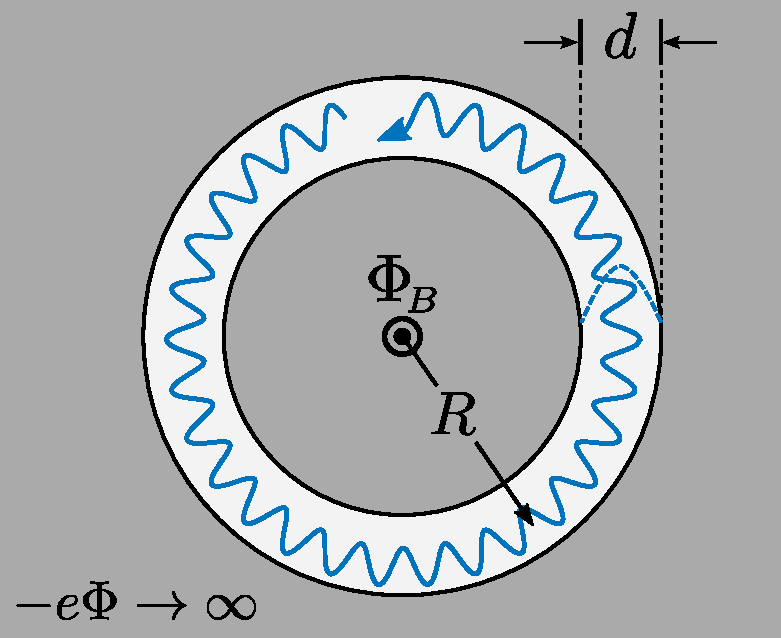
\includegraphics[width=0.4\textwidth]{annulus}
\end{figure}

Now, suppose we thread magnetic flux (e.g., using a solenoid) through
the origin, which lies in the region enclosed by the annulus.  This
flux can be described via the vector potential
\begin{equation}
  \mathbf{A}(r,\phi) = \frac{\Phi_B}{2\pi r} \, \hat{e}_\phi.
  \label{Asolenoid}
\end{equation}
We can verify from Eq.~\eqref{Asolenoid} that the magnetic flux
through any loop of radius $r$ enclosing the origin is $(\Phi_B/2\pi
r)(2\pi r) = \Phi_B$, independent of $r$.  Hence, the magnetic flux is
confined to an infintesimal area surrounding the origin, with
$\mathbf{B} = 0$ everywhere else. The vector potential $\mathbf{A}$,
however, is nonzero everywhere.

The time-independent Schr\"odinger equation is
\begin{equation}
  \frac{1}{2m}\left|-i\hbar\nabla+
  \frac{e\Phi_B}{2\pi r} \, \hat{e}_\phi\right|^2 \psi(r,\phi)
  = E\psi(r,\phi),
  \label{ABschrod}
\end{equation}
with the boundary conditions $\psi(R\pm d/2,0) = 0$.  For sufficiently
large $R$, we can guess that the eigenfunctions have the form
\begin{equation}
  \psi(r,\phi) \approx
  \psi_0 \, \cos\left(\frac{\pi}{d}(r-R)\right)\, e^{i k R \phi},
\end{equation}
where $\psi_0$ is a normalization constant.  This describes a waveform
with a half-wavelength wave profile in the $r$ direction (so as to
vanish at $r = R \pm d/2$), and traveling along the azimuthal
direction with wavenumber $k$.  In order for the wavefunction to be
single-valued,
\begin{equation}
  k \cdot 2\pi R = 2\pi n \;\;\;\Rightarrow \;\;\; k = \frac{n}{R},
  \;\;\;\mathrm{where}\;\; n \in \mathbb{Z}.
\end{equation}
Plugging this into Eq.~\eqref{ABschrod} yields the energy levels
\begin{align}
  E_n &= \frac{1}{2m} \left[
    \left(\frac{n\hbar}{R} + \frac{e\Phi_B}{2\pi R}\right)^2
    + \left(\frac{\pi\hbar}{d}\right)^2 \right] \\
  &= \frac{e^2}{8\pi^2mR^2} \left(\Phi_B + \frac{nh}{e} \right)^2
  + \frac{\pi^2\hbar^2}{2md^2}.
  \label{abcurves}
\end{align}
In the figure below, these energy levels are sketched versus the
magnetic flux $\Phi_B$.  According to Eq.~\eqref{abcurves}, the
energies are described by a set of quadratic curves, translated along
the $\Phi_B$ axis by integer multiples of $h/e$.  Evidently, varying
$\Phi_B$ will shift the eigen-energies in the annulus, despite the
fact that the magnetic field vanishes in the annulus.  This is a
manifestation of the Aharonov-Bohm effect.

\begin{figure}[h]
  \centering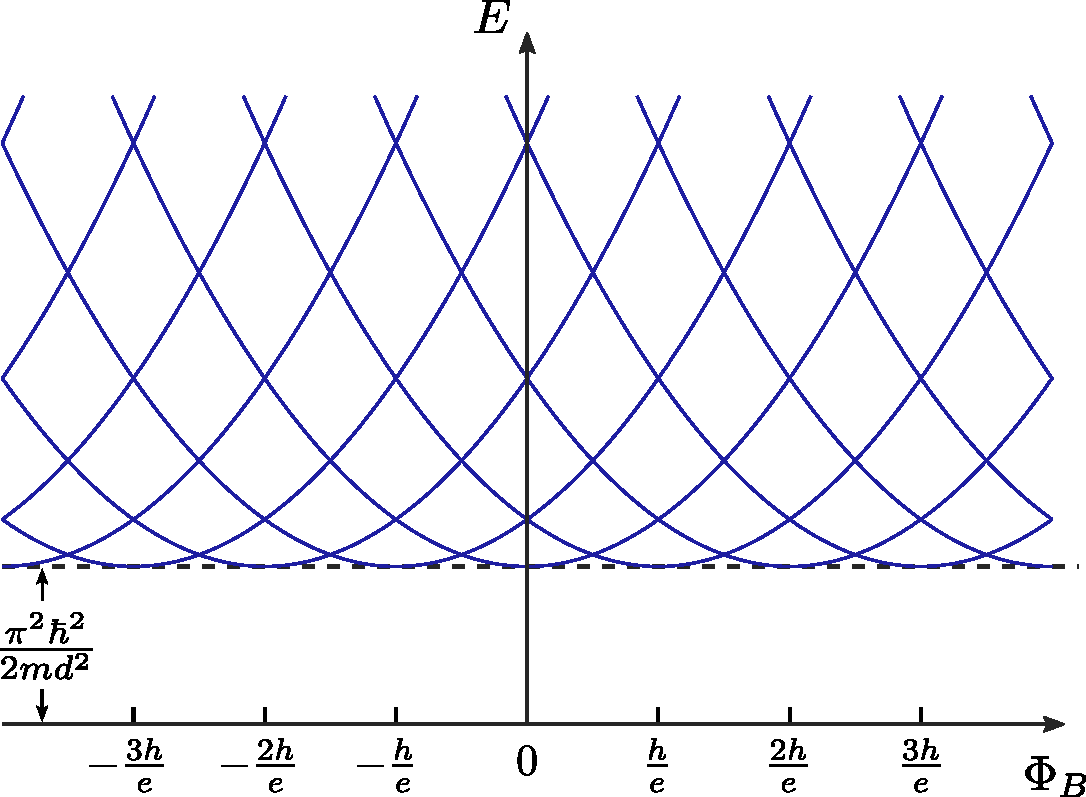
\includegraphics[width=0.65\textwidth]{abring}
\end{figure}

One very interesting feature of this energy spectrum is that it
remains the same whenever the magnetic flux changes by an exact
multiple of $h/e = 4.13567\times10^{-5}\,\mathrm{T}\,\mathrm{m}^2$.
This fundamental unit of magnetic flux is called the \textbf{magnetic
  flux quantum}.  Notably, it does not depend on the radius of the
annulus, or any other geometrical parameters of the system.  This is
because the invariance property arises from the gauge symmetry of the
Hamiltonian.  When an extra flux of $nh/e$ (where $n\in\mathbb{Z}$) is
threaded through the annulus, Eq.~\eqref{Asolenoid} tells us that the
change in vector potential is $\Delta \mathbf{A} = (n\hbar/ e r)
\hat{e}_\phi$.  We can undo the effects of this additional vector
potential using the gauge field
\begin{equation}
  \lambda(r,\phi) = \frac{n\hbar}{e} \, \phi \;\;\;\Rightarrow
  \begin{cases}\nabla \lambda &= \displaystyle (n\hbar/er) \hat{e}_\phi
    \\ \displaystyle e^{ie\lambda/\hbar} &= \displaystyle e^{in\phi}.
  \end{cases}
\end{equation}
Note that this gauge field is not single-valued, but it's not a
problem since both $\nabla\lambda$ and the phase factor
$\exp(ie\lambda/\hbar)$ remain single-valued.

\subsection{The Dirac Hamiltonian}
\label{sec:DiracH}

The $p^2/2m$-type Hamiltonians we have been dealing with describe
non-relativistic particles.  In 1928, Paul Dirac formulated a new type
of Hamiltonian that can be used to describe particles moving close to
the speed of light, thus successfully combining quantum mechanics with
the special theory of relativity. Another triumph of Dirac's theory is
that after including electromagnetic scalar and vector potentials
(following the procedures discussed in Sec.~\ref{sec:nonrel}), it
accurately predicts the magnetic moment of the electron.

To formulate Dirac's Hamiltonian, we start from the time-dependent
Schr\"odinger equation.  In the wavefunction representation, this has
the form
\begin{equation}
  i\hbar\, \partial_t\, \psi(\mathbf{r},t)
  = \hat{H} \psi(\mathbf{r},t).
\end{equation}
Note that the left side has a first-order time derivative.  On the
right side, the Hamiltonian $\hat{H}$ contains spatial derivatives.
We know that time and space derivatives of wavefunctions are related
to energy and momentum by
\begin{equation}
    i\hbar\, \partial_t\; \leftrightarrow \;
    E, \qquad
    -i\hbar\, \partial_j \;\leftrightarrow \;
    p_j.
\end{equation}
We also know that the energy and momentum of a relativistic particle
are related by
\begin{equation}
  E^2 = m^2c^4 + \sum_{j=1}^3 p_j^2c^2,
  \label{Erelativistic}
\end{equation}
where $m$ is the rest mass and $c$ is the speed of light.  (Following
the usual practice in relativity theory, we use Roman indices $j \in
\{1,2,3\}$ for the spatial coordinates $\{x,y,z\}$.)  In
Eq.~\eqref{Erelativistic}, $E$ and $p$ appear to the same
order---unlike the non-relativistic kinetic energy $E = p^2/2m$, where
$E$ is first-order while $p$ is second-order.  Since the left side of
the Schr\"odinger equation has a first-order time derivative, a
relativistic Hamiltonian $\hat{H}$ ought to contain only first-order
spatial derivatives.  So we make the guess
\begin{equation}
  \hat{H} = \alpha_0 mc^2 + \sum_{j=1}^3 \alpha_j \hat{p}_j c,
  \label{Dirac0}
\end{equation}
where $\hat{p}_j \equiv -i\hbar \partial/\partial x_j$ is the usual
momentum operator.  We now need to determine the ``coefficients''
$\alpha_0$, $\alpha_1$, $\alpha_2$, and $\alpha_3$.  The extra factors
of $mc^2$ and $c$ are included in Eq.~\eqref{Dirac0} for later
convenience.

For a wavefunction with definite momentum $\mathbf{p}$ and energy
$E$,
\begin{equation}
  \hat{H}\psi = E \psi \;\;\;\Rightarrow \;\;\;
  \left(\alpha_0mc^2 + \sum_{j=1}^3\alpha_j p_jc\right) \psi = E\,\psi,
\end{equation}
where the $\hat{p}_j$ operators are replaced with definite numbers.
If $\psi$ is a scalar, this would imply that $\alpha_0 mc^2 +
\sum_{j}\alpha_j p_j c = E$, which does not match the relativistic
energy-mass-momentum relation \eqref{Erelativistic}.  However, we can
get it to work if the $\alpha$'s are matrices rather than numbers:
\begin{equation}
\boxed{\qquad \hat{H} = \hat{\alpha}_0 mc^2 + \sum_{j=1}^3 \hat{\alpha}_j \hat{p}_j c, \;\; \mathrm{where}\;\; \hat{p}_j \equiv -i\hbar\, \partial_j.\qquad}
\label{Dirac}
\end{equation}
In that case, applying the Hamiltonian twice gives
\begin{equation}
  \left(\hat{\alpha}_0mc^2 + \sum_{j=1}^3\hat{\alpha}_j p_j c\right)^{\!2}\;
  \psi = E^2\,\psi.
\end{equation}
This can be satisfied if
\begin{equation}
  \left(\hat{\alpha}_0 mc^2 + \sum_{j=1}^3\hat{\alpha}_j p_j c\right)^2
  = E^2\, \hat{I},
\end{equation}
where $\hat{I}$ is the identity matrix.  Expanding the square (and
taking care of the fact that the $\hat{\alpha}_\mu$ matrices need not
commute) yields
\begin{equation}
  \hat{\alpha}_0^2 m^2c^4
  + \sum_j \left(\hat{\alpha}_0 \hat{\alpha}_j + \hat{\alpha}_j \hat{\alpha}_0\right) mc^3 p_j
  + \sum_{jj'} \left(\hat{\alpha}_j \hat{\alpha}_{j'} + \hat{\alpha}_{j'} \hat{\alpha}_j\right) p_j p_{j'} = E^2\hat{I}.
\end{equation}
This reduces to Eq.~\eqref{Erelativistic} if the $\hat{\alpha}_\mu$
matrices satisfy
\begin{align}
  \begin{aligned}
    \hat{\alpha}_\mu^2 &= \hat{I} \;\;\; \textrm{for} \;\;\mu=0,1,2,3,
    \;\;\textrm{and} \\
    \hat{\alpha}_\mu \hat{\alpha}_\nu
    + \hat{\alpha}_\nu \hat{\alpha}_\mu &= 0
    \;\;\; \textrm{for} \;\;\mu \ne \nu.
  \end{aligned}
\end{align}
(Here, we adopt the usual relativistic convention of using Greek
symbols to label indices ranging over $\{0,1,2,3\}$.)  The above can
be written more concisely using the anticommutator notation,
$\{\hat{A},\hat{B}\} \equiv \hat{A}\hat{B} + \hat{B}\hat{A}$:
\begin{equation}
  \{\hat{\alpha}_\mu, \hat{\alpha}_\nu\} = 2\delta_{\mu\nu},
  \;\;\; \textrm{for} \;\;\mu,\nu=0,1,2,3,
  \label{Dirac_anticomm}
\end{equation}
Also, we need the $\hat{\alpha}_\mu$ matrices to be Hermitian, so that
$\hat{H}$ is Hermitian.

It turns out that the smallest possible Hermitian matrices that can
satisfy Eq.~\eqref{Dirac_anticomm} are $4\times4$ matrices.  The
choice of matrices is not uniquely determined; a commonly used set is
\begin{align}
  \begin{aligned}
    \hat{\alpha}_0 &= \begin{bmatrix}
      \hat{I}\, & \hat{0} \\ \hat{0} & -\hat{I}
    \end{bmatrix}, \;\;\;
    \hat{\alpha}_1 = \begin{bmatrix}
      \hat{0} & \hat{\sigma}_1 \\ \hat{\sigma}_1 & \hat{0}
    \end{bmatrix} \\
    \hat{\alpha}_2 &= \begin{bmatrix}
      \hat{0} & \hat{\sigma}_2 \\ \hat{\sigma}_2 & \hat{0}
    \end{bmatrix}, \;\;\;
    \hat{\alpha}_3 = \begin{bmatrix}
      \hat{0} & \hat{\sigma}_3 \\ \hat{\sigma}_3 & \hat{0}
    \end{bmatrix},
  \end{aligned}
  \label{alpha_matrices}
\end{align}
where $\{\hat{\sigma}_{1}, \hat{\sigma}_{2}, \hat{\sigma}_{3}\}$
denote the usual Pauli matrices.  It follows also that
$\psi(\mathbf{r})$ cannot be a scalar field, but must be a
four-component field.

\subsection{Eigenstates of the Dirac Hamiltonian}

According to Eq.~\eqref{Erelativistic}, the energy eigenvalues of the
Dirac Hamiltonian are
\begin{equation}
  E = \pm \sqrt{m^2c^4 + \sum_{j} p_j^2c^2}.
\end{equation}

\pagebreak

As shown in the figure below, the energy spectrum forms two ``bands''.
For any given momentum $\mathbf{p}$, there is a positive value of $E$,
and a negative value.

\begin{center}
  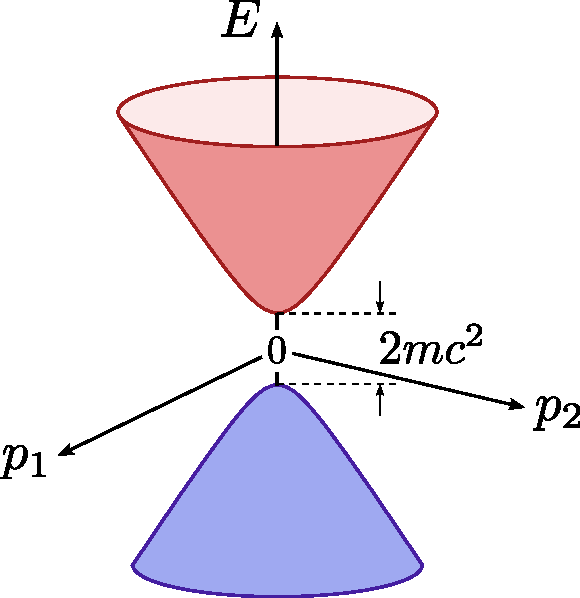
\includegraphics[width=0.3\textwidth]{diraccone}
\end{center}

The upper band matches the dispersion relation for a massive
relativistic particle, which is what we were originally after.
However, there is also a band of negative-energy states---who ordered
that?!  So long as we are considering a single isolated electron, we
can simply declare that the positive-energy states are the ones we are
interested in.  However, once we couple the electron to the
electromagnetic field, the existence of the negative-energy states
points to a nonsensical scenario.  The negative-energy band extends
down to $E \rightarrow -\infty$, which means the system has no ground
state.  This implies that the electron can keep losing energy by
photon emission, forever hopping to ever-lower-energy states!

The resolution of this problem is an interesting story, but one we
will not be able to pursue in this course.  Basically, we now know
that Dirac's original theory contains the seeds of its own
destruction, since a consistent theory of \textit{single-particle}
relativistic quantum mechanics is ultimately impossible.  The right
way to marry relativity and quantum mechanics is to use the framework
of quantum field theory, which is capable of describing states with
arbitrary numbers of electrons and photons.  When the Dirac
Hamiltonian is translated into this framework, and coupled to a
quantized electromagnetic field, the resulting theory of quantum
electrodynamics (QED) is more well-behaved, and constitutes the most
fundamental and successful theory of electromagnetism known to date.

Let us put such issues aside for now, and do a bit more analysis on
the eigenstates of the single-particle Dirac Hamiltonian.  Since the
Hamiltonian supports two bands of solutions, there must be an even
number of wavefunction components: one set for the quantum amplitudes
of the upper band, and the other for the lower band.

Within each band, there is another two-fold degree of freedom.  This
turns out to describe the particle's spin (we are already familiar
with the use of two-component wavefunctions to describe spin-$1/2$
non-relativistic particles).  Hence, the number of components is
$2\times2 = 4$.  It is noteworthy that we did not set out to include
spin in the theory, yet it has popped up, seemingly unavoidably, in
the process of satisfying the relativistic energy-mass-momentum
relation!  This is an indicator that relativistic quantum mechanics is
more ``theoretically rigid'' than non-relativistic quantum mechanics.
Features like spin are not optional parts of the theory, but have to
be included at a fundamental level.

Different choices of the $\hat{\alpha}_\mu$ matrices correspond to
different wavefunction representations, similar to the choice of
spin-$1/2$ basis in the non-relativistic theory.  The matrices in
Eq.~\eqref{alpha_matrices} are designed so that they reduce to the
non-relativistic limit in a nice way.  Upon plugging them into
Eq.~\eqref{Dirac}, we find that for an eigenstate with energy $E$ and
momentum $\mathbf{p}$,
\begin{align}
  \psi = \begin{bmatrix}\psi_A \\ \psi_B
  \end{bmatrix}, \;\;\;\mathrm{where}\;\;\; \left\{
  \begin{aligned}
    \psi_A &= \frac{1}{E - mc^2} \sum_j \hat{\sigma}_j p_j \psi_B, \\
    \psi_B &= \frac{1}{E + mc^2} \sum_j \hat{\sigma}_j p_j \psi_A.
  \end{aligned}\right.
  \label{dirac_nonrelativistic}
\end{align}
Hence, in the non-relativistic limit, for the upper band ($E \gtrsim
mc^2$) the wavefunction is dominated by the two upper components
($|\psi_B| \rightarrow 0$); and for the lower band ($E \lesssim
-mc^2$) the wavefunction is dominated by the two lower components
($|\psi_A| \rightarrow 0$).  The two non-negligible wavefunction
components for each band then describe the spin-$1/2$ degree of
freedom.  (However, please note that this clean grouping into ``upper
band'' and ``lower band'' components only works in the
non-relativistic limit!  In the relativistic case, upper band states
acquire non-vanishing values in the lower two wavefunction components,
and vice versa.)

There is much more to be said about the structure and interpretation
of the Dirac Hamiltonian and its wavefunction, especially the
important issue of how they behave under rotations and Lorentzian
transformations.  For these details, the reader is referred to
\hyperref[cite:dyson]{Dyson (1951)}.

\subsection{Electrons in an electromagnetic field}
\label{sec:diracem}

Having obtained a Hamiltonian that describes the relativistic dynamics
of a electron, we are naturally interested in putting the electron in
an electromagnetic field.  The non-relativistic theory from
Section~\ref{sec:nonrel} allows us to guess how to do this.  There, we
simply added $-e\Phi(\mathbf{r},t)$ as a scalar potential function,
and inserted the vector potential via the substitution
\begin{equation}
  \hat{\mathbf{p}} \rightarrow \hat{\mathbf{p}}
  + e\mathbf{A}(\hat{\mathbf{r}},t).  
\end{equation}
If we apply the same procedure to the Dirac Hamiltonian (\ref{Dirac}),
the result is
\begin{equation}
  i\hbar \, \partial_t \psi
  = \left\{\hat{\alpha}_0 mc^2 -e\Phi(\mathbf{r},t)
  + \sum_{j} \hat{\alpha}_j \Big[-i\hbar\,\partial_j
    +eA_j(\mathbf{r},t) \Big] c\right\}\psi(\mathbf{r},t).
\end{equation}
Using the $\hat{\alpha}_\mu$ matrices from Eq.~\eqref{alpha_matrices},
this reduces to a pair of two-component equations:
\begin{align}
  i\hbar\, \partial_t \, \psi_A
  &= \big(+mc^2 -e\Phi \big)\,
  \psi_A
  \,+\, \sum_{j} \hat{\sigma}_j \big(-i\hbar\partial_j
    +eA_j \big) \,c\;\psi_B \label{Dirac2a} \\
  i\hbar\, \partial_t \, \psi_B
  &= \big(- mc^2 -e\Phi\big)\,
  \psi_B \,+\, \sum_{j} \hat{\sigma}_j \big(-i\hbar\partial_j
    +eA_j \big)\, c\;\psi_A, \label{Dirac2b}
\end{align}
where $\psi_A(\mathrm{r},t)$ and $\psi_B(\mathrm{r},t)$ are upper and
lower wavefunction components, like in
Eq.~\eqref{dirac_nonrelativistic}.

An extremely important result is obtained by taking the
non-relativistic limit of the above equations.  In this limit, we look
for solutions in the ``slowly-varying envelope approximation''
\begin{equation}
  \psi_{A/B}(\mathbf{r},t) = \Psi_{A/B}(\mathbf{r},t)\,
  \exp\left[-i\left(\frac{mc^2}{\hbar}\right)t\right].
\end{equation}
The exponential on the right side is the $\exp(-i\omega t)$ factor
corresponding to the rest energy $mc^2$, which is the dominant
contribution to the electron's energy in the non-relativistic limit.
The two-component ``envelope'' functions $\Psi_A$ and $\Psi_B$ vary
slowly in $t$ compared to the exponential factor.  Note that by
putting $mc^2$ rather than $-mc^2$ in the exponential factor, we are
explicitly looking for positive-energy solutions.

Plugging this ansatz into Eqs.~\eqref{Dirac2a}--\eqref{Dirac2b} gives
\begin{align}
  i\hbar\, \partial_t \, \Psi_A
  &= -e\Phi\; \Psi_A
  \,+\, \sum_{j} \hat{\sigma}_j \big(-i\hbar\partial_j
    +eA_j \big) c\;\Psi_B \label{Dirac3a} \\
  \big(i\hbar\, \partial_t \, + 2mc^2 + e\Phi\big)
  \Psi_B
  &= \sum_{j} \hat{\sigma}_j \big(-i\hbar\partial_j
    +eA_j \big) c\;\Psi_A. \label{Dirac3b}
\end{align}
On the left side of Eq.~\eqref{Dirac3b}, the $2mc^2$ term dominates
over the other two, so
\begin{equation}
  \Psi_B \;\approx\; \frac{1}{2mc}\, \sum_{j}
  \hat{\sigma}_j \big(-i\hbar\partial_j +eA_j \big) \;\Psi_A.
\end{equation}
Plugging this into Eq.~\eqref{Dirac3a} yields
\begin{equation}
  i\hbar\, \partial_t \, \Psi_A
  = \left\{-e\Phi \,+\, \frac{1}{2m} \sum_{jk} \hat{\sigma}_j \hat{\sigma}_k
  \big(-i\hbar\partial_j +eA_j \big)
  \big(-i\hbar\partial_k +eA_k \big) \right\}\;\Psi_A.
\end{equation}
Using the identity $\hat{\sigma}_j\hat{\sigma}_k = \delta_{jk}\hat{I}
+ i \sum_i \varepsilon_{ijk}\sigma_i$:
\begin{align}
  \begin{aligned}
  i\hbar\, \partial_t \, \Psi_A
  &= \Bigg\{-e\Phi
  \,+\, \frac{1}{2m} \big|-i\hbar\nabla +e\mathbf{A} \big|^2 \\
  &\qquad+\, \frac{i}{2m} \sum_{ijk} \varepsilon_{ijk} \hat{\sigma}_i
  \big(-i\hbar\partial_j +eA_j \big)
  \big(-i\hbar\partial_k +eA_k \big)
  \Bigg\} \Psi_A.
  \end{aligned}
\end{align}
Look carefully at the last term in the curly brackets.  Expanding the
square yields
\begin{equation*}
  \frac{i}{2m}\sum_{ijk}\varepsilon_{ijk}\hat{\sigma}_i
  \Big(-\partial_j\partial_k -i\hbar e \partial_jA_k
  - i\hbar e \big[A_k\partial_j + A_j\partial_k \big]
  + e^2A_jA_k \Big).
\end{equation*}
Due to the $\varepsilon_{ijk}$, all terms that are symmetric under $j$
and $k$ will cancel out after the sums are carried out.  The only
surviving term is the second one, which yields
\begin{equation}
  \frac{\hbar e}{2m}\sum_{ijk}\varepsilon_{ijk}\hat{\sigma}_i
  \partial_jA_k = \frac{\hbar e}{2m} \hat{\boldsymbol{\sigma}}
  \,\cdot\, \mathbf{B}(\mathbf{r},t),
\end{equation}
where $\mathbf{B} = \nabla\times\mathbf{A}$ is the magnetic field.
Hence,
\begin{equation}
  i\hbar\, \partial_t \, \Psi_A
  = \left\{-e\Phi
  \,+\, \frac{1}{2m} \big|-i\hbar\nabla +e\mathbf{A} \big|^2
  \,-\, \left(-\frac{\hbar e}{2m}\, \hat{\boldsymbol{\sigma}}\right)
  \,\cdot\, \mathbf{B} \right\} \Psi_A.
\end{equation}
This is an exact match for Eq.~\eqref{quantumH}, except that the
Hamiltonian has an additional term of the form $-
\hat{\boldsymbol{\mu}} \cdot \hat{\mathbf{B}}$.  This additional term
corresponds to the potential energy of a magnetic dipole of moment
$\boldsymbol{\mu}$ in a magnetic field $\mathbf{B}$.  The Dirac theory
therefore predicts that the electron's magnetic dipole moment is
\begin{equation}
  |\boldsymbol{\mu}| = \frac{\hbar e}{2m}.
  \label{Diracmu}
\end{equation}
This remarkable result matches the experimentally-observed magnetic
dipole moment to about one part in $10^3$.  We thus see that the
electron's magnetic dipole moment is not an arbitrary quantity, but an
outcome of combining quantum mechanics with relativity.  The residual
mismatch between Eq.~\eqref{Diracmu} and the actual magnetic dipole
moment of the electron is understood to arise from quantum
fluctuations of the electronic and electromagnetic quantum fields;
this ``anomalous magnetic moment'' can be calculated using the full
QED theory, and matches experiment to around one part in $10^9$,
making it one of the most precise theoretical predictions in physics.
For details, see \hyperref[cite:zee]{Zee (2010)}.

\section{Quantizing the electromagnetic field}
\label{sec:em_quantization}

We have previously seen how to quantize a simple scalar boson field
(Chapter 3, Sec.~V.C): the classical field is decomposed into normal
modes, and each mode is quantized by treating it as an independent
oscillator, with its own creation and annihilation operators.  By
comparing the oscillator energies in the classical and quantum
regimes, we derive the Hermitian operator corresponding to the
classical field variable, expressed in terms of the creation and
annihilation operators.

We will use this approach, with minor adjustments, to quantize the
electromagnetic field.

First, consider a ``source-free'' electromagnetic field---i.e., with
no electric charges and currents.  Without sources, Maxwell's
equations (in SI units, and in a vacuum) reduce to:
\begin{align}
  \nabla\cdot \mathbf{E} &= 0 \label{max1} \\
  \nabla\cdot \mathbf{B} &= 0 \label{max2}\\
  \nabla\times \mathbf{E} &= -\frac{\partial \mathbf{B}}{\partial t} \label{max3}\\
  \nabla\times \mathbf{B} &= \frac{1}{c^2} \frac{\partial \mathbf{E}}{\partial t}.
  \label{max4}
\end{align}
Once again, we introduce the scalar potential $\Phi$ and vector
potential $\mathbf{A}$:
\begin{align}
  \mathbf{E} &= - \nabla \Phi - \frac{\partial\mathbf{A}}{\partial t} \\
  \mathbf{B} &= \nabla \times \mathbf{A}.
\end{align}
These relations cause Eqs.~\eqref{max2} and \eqref{max3} to be
satisfied automatically, via vector identities.  The other two Maxwell
equations, \eqref{max1} and \eqref{max4}, become:
\begin{align}
  \nabla^2 \Phi &= -\frac{\partial}{\partial t} \nabla \cdot \mathbf{A} \label{max5} \\
  \left(\nabla^2 - \frac{1}{c^2}\frac{\partial^2}{\partial t^2}\right)
  \mathbf{A} &= \nabla\left[\frac{1}{c^2}\frac{\partial}{\partial t}  \Phi + \nabla\cdot\mathbf{A}\right]. \label{max6}
\end{align}

In the next step, we choose a convenient gauge called the
\textbf{Coulomb gauge}:
\begin{equation}
  \Phi = 0, \;\;\; \nabla \cdot \mathbf{A} = 0.
  \label{coulomb}
\end{equation}
(To see that we can always make such a gauge choice, suppose we start
out with a scalar potential $\Phi_0$ and vector potential
$\mathbf{A}_0$ not satisfying \eqref{coulomb}.  Perform a gauge
transformation with a gauge field $\lambda(\mathbf{r}, t) = - \int^t
dt'\; \Phi_0(\mathbf{r}, t')$.  Then the new scalar potential is $\Phi
= \Phi_0 + \dot{\lambda} = 0$; moreover, the new vector potential
satisfies
\begin{equation}
  \nabla\cdot\mathbf{A} = \nabla\cdot \mathbf{A}_0 - \nabla^2 \lambda
  = \nabla\cdot \mathbf{A}_0 + \int^t dt'\; \nabla^2\Phi_0(\mathbf{r}, t').
\end{equation}
Upon using Eq.~\eqref{max5}, we find that $\nabla\cdot\mathbf{A} =
0$.)

In the Coulomb gauge, Eq.~\eqref{max5} is automatically satisfied.
The remaining equation, \eqref{max6}, simplifies to
\begin{equation}
  \left(\nabla^2 - \frac{1}{c^2}\frac{\partial^2}{\partial t^2}\right)
  \mathbf{A} = 0. \label{max8}
\end{equation}
Hence, we deduce that the normal modes are \textbf{light waves} that
have the plane-wave form
\begin{equation}
  \mathbf{A}(\mathbf{r},t) = \Big(\mathcal{A}\,
  \, e^{i(\mathbf{k}\cdot\mathbf{r} - \omega t)} + \mathrm{c.c.}\Big)\, \hat{e},
  \label{lightplanewave}
\end{equation}
where $\mathcal{A}$ is a complex number (the \textbf{mode amplitude})
that specifies the magnitude and phase of the plane wave, $\hat{e}$ is
a real unit vector (the \textbf{polarization vector}) that specifies
which direction the vector potential points along, and
``c.c.''~denotes the complex conjugate of the first term.  Referring
to Eq.~\eqref{max8}, we see that the frequency $\omega$ must satisfy
\begin{equation}
  \omega = c|\mathbf{k}|.
\end{equation}
For convenience, suppose for now that we put the electromagnetic field
in a box of volume $V = L^3$, with periodic boundary conditions, so
that the $\mathbf{k}$ vectors form a discrete set:
\begin{equation}
  k_j = \frac{2\pi n_j}{L}, \;\; n_j \in \mathbf{Z}, \;\;\mathrm{for}
  \;\; j = 1,2,3.
\end{equation}
We will take the $L \rightarrow \infty$ limit at the very end.

Since $\nabla \cdot \mathbf{A} = 0$, it must also be the case that
\begin{equation}
  \mathbf{k} \cdot \hat{e} = 0.
\end{equation}
In other words, the polarization vector is perpendicular to the
propagation direction.  For each $\mathbf{k}$, there are two
orthogonal polarization, which can be labelled by an index $\lambda =
1,2$.

Hence, the vector potential field can be generally decomposed into a
discrete superposition of plane waves:
\begin{equation}
  \mathbf{A}(\mathbf{r},t) = \sum_{\mathbf{k}\lambda} 
  \Big(\mathcal{A}_{\mathbf{k}\lambda} \, e^{i(\mathbf{k}\cdot\mathbf{r} - \omega_{\mathbf{k}} t)}
  + \mathrm{c.c.}\Big)\, \hat{e}_{\mathbf{k}\lambda},
  \;\;\; \mathrm{where}
  \;\;\;\omega_{\mathbf{k}} = c|\mathbf{k}|.
\end{equation}
To convert the classical field theory into a quantum field theory, for
each $(\mathbf{k},\lambda)$ we define an independent set of creation
and annihilation operators:
\begin{equation}
  \big[\hat{a}_{\mathbf{k}\lambda}, \hat{a}_{\mathbf{k}'\lambda'}^\dagger\big]
  = \delta_{\mathbf{k}\mathbf{k}'} \delta_{\lambda\lambda'}, \;\;\;
  \big[\hat{a}_{\mathbf{k}\lambda}, \hat{a}_{\mathbf{k}'\lambda'}\big]
  = \big[\hat{a}_{\mathbf{k}\lambda}^\dagger, \hat{a}_{\mathbf{k}'\lambda'}^\dagger\big]
  = 0.
\end{equation}
Then the Hamiltonian for the electromagnetic field is
\begin{equation}
  \hat{H} = \sum_{\mathbf{k}\lambda} \hbar \omega_{\mathbf{k}} \,
  \hat{a}^\dagger_{\mathbf{k}\lambda} \hat{a}_{\mathbf{k}\lambda},
  \;\;\; \mathrm{where}
  \;\;\;\omega_{\mathbf{k}} = c|\mathbf{k}|.
\end{equation}
And the vector potential is promoted into a Hermitian operator in the
Heisenberg picture:
\begin{equation}
  \hat{\mathbf{A}}(\mathbf{r},t) = \sum_{\mathbf{k}\lambda} 
  \mathcal{C}_{\mathbf{k}\lambda}\,
  \Big(\hat{a}_{\mathbf{k}\lambda} \, e^{i(\mathbf{k}\cdot\mathbf{r} - \omega_{\mathbf{k}} t)}
  + \mathrm{h.c.}\Big)\, \hat{e}_{\mathbf{k}\lambda}.
\end{equation}
Here, $\mathcal{C}_{\mathbf{k}\lambda}$ is a constant to be
determined, and ``h.c.''~denotes the Hermitian conjugate.  The
creation and annihilation operators in this equation are Schr\"odinger
picture ($t = 0$) operators (see Chapter 3, Sec.~V.C).  The particles
that they create/annihilate are called \textbf{photons}---elementary
particles of light.

To find $\mathcal{C}_{\mathbf{k}\lambda}$, we compare the quantum and
classical energies.  Consider the quantum case first: suppose the
electromagnetic field is in a coherent state
$|\alpha_{\mathbf{k}\lambda}\rangle$ such that
\begin{equation}
  \hat{a}_{\mathbf{k}\lambda}|\alpha_{\mathbf{k}\lambda}\rangle
  = \alpha_{\mathbf{k}\lambda}|\alpha_{\mathbf{k}\lambda}\rangle,
  \label{coherent}
\end{equation}
for some $\alpha_{\mathbf{k}\lambda} \in \mathbb{C}$.  Then the mean
squared expectation value of $A^2$, where $A$ is the vector potential
component parallel to the polarization vector
$\hat{e}_{\mathbf{k}\lambda}$, is
\begin{equation}
  \overline{\langle \alpha_{\mathbf{k}\lambda} | \hat{A}^2(\mathbf{r},t) | \alpha_{\mathbf{k}\lambda}\rangle}
  = 2 \, |\mathcal{C}_{\mathbf{k}\lambda}|^2 \, |\alpha_{\mathbf{k}\lambda}|^2.
  \label{quant_Asq}
\end{equation}
The energy is
\begin{equation}
  E = \hbar\omega_{\mathbf{k}} |\alpha_{\mathbf{k}\lambda}|^2.
  \label{quant_energy}
\end{equation}

Now compare this to the classical case.  The energy density (energy
per unit volume) of a classical source-free electromagnetic plane wave
is
\begin{equation}
  \overline{u} = \varepsilon_0\, \omega^2 \, \overline{A^2},
\end{equation}
where $\varepsilon_0$ is the permittivity of free space.  Combining
this with Eqs.~\eqref{quant_Asq} and \eqref{quant_energy}, and taking
$E = \overline{u} V$, yields
\begin{align}
  \hbar\omega_{\mathbf{k}} |\alpha_{\mathbf{k}\lambda}|^2 &=
  \left(\varepsilon_0\, \omega^2\right) \,
  \left(2 \, |\mathcal{C}_{\mathbf{k}\lambda}|^2 \, |\alpha_{\mathbf{k}\lambda}|^2\right)\, V \\
  \Rightarrow \quad \mathcal{C}_{\mathbf{k}\lambda} &= \sqrt{\frac{\hbar}{2\varepsilon_0\omega_{\mathbf{k}}V}}.
\end{align}
We thus arrive at the result
\begin{align}
\boxed{\qquad
  \begin{aligned}
    \hat{H} &= \sum_{\mathbf{k}\lambda} \hbar \omega_{\mathbf{k}} \,
    \hat{a}^\dagger_{\mathbf{k}\lambda} \hat{a}_{\mathbf{k}\lambda} \\
  \hat{\mathbf{A}}(\mathbf{r},t) &= \sum_{\mathbf{k}\lambda} 
  \sqrt{\frac{\hbar}{2\varepsilon_0\omega_{\mathbf{k}}V}}\,
  \Big(\hat{a}_{\mathbf{k}\lambda} \, e^{i(\mathbf{k}\cdot\mathbf{r} - \omega_{\mathbf{k}} t)}
  + \mathrm{h.c.}\Big)\, \hat{e}_{\mathbf{k}\lambda} \\
  \omega_{\mathbf{k}} &= c|\mathbf{k}|,  \;\;\;
  \big[\hat{a}_{\mathbf{k}\lambda}, \hat{a}_{\mathbf{k}'\lambda'}^\dagger\big]
  = \delta_{\mathbf{k}\mathbf{k}'} \delta_{\lambda\lambda'}, \;\;\;
  \big[\hat{a}_{\mathbf{k}\lambda}, \hat{a}_{\mathbf{k}'\lambda'}\big]
  = 0.
  \end{aligned}
  \qquad}
  \label{qed1}
\end{align}
To describe infinite free space rather than a finite-volume box, we
take the $L\rightarrow \infty$ limit and re-normalize the creation and
annihilation operators by the replacement
\begin{equation}
  \hat{a}_{\mathbf{k}\lambda} \rightarrow \sqrt{\frac{(2\pi)^3}{V}} \;
  \hat{a}_{\mathbf{k}\lambda}.
\end{equation}
Then the sums over $\mathbf{k}$ become integrals over the infinite
three-dimensional space:
\begin{align}
\boxed{\qquad
  \begin{aligned}
    \hat{H} &= \int d^3k\sum_{\lambda} \hbar \omega_{\mathbf{k}} \,
    \hat{a}^\dagger_{\mathbf{k}\lambda} \hat{a}_{\mathbf{k}\lambda} \\
  \hat{\mathbf{A}}(\mathbf{r},t) &= \int d^3k \sum_{\lambda} 
  \sqrt{\frac{\hbar}{16\pi^3\varepsilon_0\omega_{\mathbf{k}}}}\,
  \Big(\hat{a}_{\mathbf{k}\lambda} \, e^{i(\mathbf{k}\cdot\mathbf{r} - \omega_{\mathbf{k}} t)}
  + \mathrm{h.c.}\Big)\, \hat{e}_{\mathbf{k}\lambda} \\
  \omega_{\mathbf{k}} &= c|\mathbf{k}|,  \;\;\;
  \big[\hat{a}_{\mathbf{k}\lambda}, \hat{a}_{\mathbf{k}'\lambda'}^\dagger\big]
  = \delta^3(\mathbf{k}-\mathbf{k}') \delta_{\lambda\lambda'}, \;\;\;
  \big[\hat{a}_{\mathbf{k}\lambda}, \hat{a}_{\mathbf{k}'\lambda'}\big]
  = 0.
  \end{aligned}
  \qquad}
  \label{qed2}
\end{align}

\section{The electron-photon interaction}

Now that we have separate quantum theories for the electron and the
electromagnetic field, we can put them together into a theory of
\textbf{quantum electrodynamics}.  This theory will be able to
describe processes involving electrons interacting with the
electromagnetic field by absorbing and/or radiating photons.

In concrete terms, let $\mathscr{H}_{\mathrm{e}}$ denote the Hilbert
space for one electron (for now, we'll use a single-particle rather
than field-theoretical description for the electron).  Let
$\mathscr{H}_{\mathrm{EM}}$ denote the Hilbert space for the
electromagnetic field (i.e., a Fock space for photons).  The states of
the combined system lie in the product space
\begin{equation*}
  \mathscr{H}_e \otimes \mathscr{H}_{\mathrm{EM}}.
\end{equation*}
We seek a Hamiltonian of the form
\begin{equation}
  H = H_e + H_{\mathrm{EM}} + H_{\mathrm{int}},
\end{equation}
where $H_e$ is the Hamiltonian for the ``bare'' electron (either an
ordinary $p^2/2m$-type Hamiltonian, or the Dirac Hamiltonian described
in Section~\ref{sec:DiracH}); $H_{\mathrm{EM}}$ is the Hamiltonian for
the source-free electromagnetic field (derived in
Section~\ref{sec:em_quantization}); and $H_{\mathrm{int}}$ is an
\textbf{interaction Hamiltonian} describing how the electron interacts
with photons.

We can use the discussion in the previous sections as a guide to
finding $H_{\mathrm{int}}$.  Let us once again adopt the Coulomb
gauge, so that the scalar potential is zero, and the electromagnetic
field is solely described via the vector potential.  In
Section~\ref{sec:nonrel}, we saw that the effect of the vector
potential on a charged particle can be described via the substitution
\begin{equation}
  \hat{\mathbf{p}} \rightarrow \hat{\mathbf{p}} +
  e\mathbf{A}(\hat{\mathbf{r}},t).
\end{equation}
In Section~\ref{sec:diracem}, we saw that this substitution is
applicable not just to non-relativistic particles, but also to fully
relativistic particles described by the Dirac Hamiltonian.
Previously, we have treated the $\mathbf{A}$ in this substitution as a
classical object lacking quantum dynamics of its own.  Now, we replace
it by the vector potential \textit{operator} derived in
Section~\ref{sec:em_quantization}:
\begin{equation}
  \hat{\mathbf{A}}(\hat{\mathbf{r}},t) =
  \begin{cases}
    \displaystyle
    \sum_{\mathbf{k}\lambda} 
  \sqrt{\frac{\hbar}{2\varepsilon_0\omega_{\mathbf{k}}V}}\,
  \Big(\hat{a}_{\mathbf{k}\lambda} \, e^{i(\mathbf{k}\cdot\mathbf{r} - \omega_{\mathbf{k}} t)}
  + \mathrm{h.c.}\Big)\, \hat{e}_{\mathbf{k}\lambda}, & (\mathrm{finite}\;\mathrm{volume}) \\
  \displaystyle \int d^3k \sum_{\lambda} 
  \sqrt{\frac{\hbar}{16\pi^3\varepsilon_0\omega_{\mathbf{k}}}}\,
  \Big(\hat{a}_{\mathbf{k}\lambda} \, e^{i(\mathbf{k}\cdot\hat{\mathbf{r}} - \omega_{\mathbf{k}} t)}
  + \mathrm{h.c.}\Big)\, \hat{e}_{\mathbf{k}\lambda},
  & (\mathrm{infinite}\;\mathrm{space}).
  \end{cases}
  \label{Aoperator}
\end{equation}

Using this, together with either the electronic and electromagnetic
Hamiltonians, we are finally able to describe the emission and
absorption of photons by electrons.  We will illustrate with a
calculation of the rate of spontaneous emission of an atom.

Suppose a non-relativistic electron is orbiting an atomic nucleus in
the excited state $|1\rangle \in \mathscr{H}_e$.  Initially, the
photon field is in its ground state, $|\varnothing\rangle \in
\mathscr{H}_{\mathrm{EM}}$.  Hence, the initial state of the combined
system is
\begin{equation}
  |\psi_i\rangle = |1\rangle \otimes |\varnothing\rangle.
\end{equation}
Let $H_{\mathrm{int}}$ be the Hamiltonian term responsible for photon
absorption/emission.  If $H_{\mathrm{int}} = 0$, then $|\psi_i\rangle$
would be an energy eigenstate.  The atom would remain in its excited
state forever.

In actuality, $H_{\mathrm{int}}$ is not zero, so $|\psi_i\rangle$ is
not an energy eigenstate.  As the system evolves, the excited electron
may decay into the ground state by emitting a photon with energy $E$,
equal to the energy difference between the atom's excited state
$|1\rangle$ and ground state $|0\rangle$.  For a non-relativistic
electron, the Hamiltonian \eqref{quantumH} yields the interaction
Hamiltonian
\begin{equation}
  H_{\mathrm{int}} = \frac{e}{2m} \left( \hat{\mathbf{p}} \cdot \hat{\mathbf{A}} + \mathrm{h.c.}\right).
\end{equation}
We will have to treat $\hat{\mathbf{A}}$ not as a classical field, but
as a field operator.

Next, consider the states that $|\psi_i\rangle$ can decay into.  There
is a continuum of possible final states, each having the form
\begin{equation}
  | \psi_{f}^{(\mathbf{k}\lambda)} \rangle = |0\rangle \otimes
  \left( \hat{a}_{\mathbf{k}\lambda}^\dagger |\varnothing\rangle\right),
  \label{decaystate}
\end{equation}
which describes the electron being in its ground state and the
electromagnetic field containing one photon, with wave-vector
$\mathbf{k}$ and polarization $\lambda$.

According to Fermi's Golden Rule (remember this?!?), the decay rate is
\begin{equation}
  \kappa = \frac{2\pi}{\hbar} \;
  \overline{\Big| \langle \psi_{f}^{(\mathbf{k}\lambda)} | \hat{H}_{\mathrm{int}}|\psi_i\rangle\Big|^2} \;
  \mathcal{D}(E),
\end{equation}
where $\overline{(\cdots)}$ denotes the average over the possible
decay states of energy $E$ (i.e., equal to the energy of the initial
state), and $\mathcal{D}(E)$ is the density of states (which has units
of inverse energy).

We therefore have to calculate the matrix element $\langle
\psi_{f}^{(\mathbf{k}\lambda)}| \hat{H}_{\mathrm{int}}|\psi_i\rangle$.
We will use the finite-volume version of the vector field operator,
Eq.~\eqref{Aoperator} (this is to avoid complications about how
Eq.~\eqref{decaystate} is to be normalized---in the finite-volume
case, we simply normalize to unity).  Moreover, in
Eq.~\eqref{Aoperator}, the $t$ dependence turns out not to matter in
this calculation, so we take $t = 0$; we also take $\hat{\mathbf{r}}
\approx 0$, which is a good approximation since the size of a typical
atomic orbital ($\sim 10^{-9}\,\textrm{m}$) is much smaller than the
optical wavelength ($\sim 10^{-6}\,\textrm{m}$).  With these
simplifications,
\begin{equation}
  \langle \psi_{f}^{(\mathbf{k}\lambda)}| \hat{H}_{\mathrm{int}}|\psi_i\rangle
  \approx \frac{e}{m} \sum_{j=1}^3 \langle 0 |\hat{p}_j|1\rangle
  \langle \varnothing| \hat{a}_{\mathbf{k}\lambda}
\left(\sum_{\mathbf{k}'\lambda'} 
  \sqrt{\frac{\hbar}{2\varepsilon_0\omega_{\mathbf{k}'}V}}\,
  \Big(\hat{a}_{\mathbf{k}'\lambda'} + \mathrm{h.c.}\Big)
  \, \hat{e}_{\mathbf{k}\lambda'}^j\right)
  |\varnothing \rangle.
  \label{matrixelt}
\end{equation}
The right side of Eq.~\eqref{matrixelt} contains two matrix elements,
one involving the electron space, and the other involving the photon
space.  The first matrix element can be simplified by observing that
for $\hat{H}_e = |\hat{\mathbf{p}}|^2/2m + V(\mathbf{r})$,
\begin{equation}
  [\hat{H}_e, \hat{\mathbf{r}}] = -i\hbar\mathbf{p}/m \;\;\;\Rightarrow \;\;\;
  \langle 0|\hat{p}_j|1\rangle = - \frac{imE \mathbf{d}}{\hbar},
\end{equation}
where $\mathbf{d} = \langle 0 |\mathbf{r} | 1\rangle$ is called the
\textbf{transition dipole moment} (note that this is generally a
complex number).  As for the photon matrix element in
\eqref{matrixelt}, the only non-vanishing elements are those of the
form
\begin{equation*}
  \langle\varnothing|\hat{a}_{\mathbf{k}\lambda} \hat{a}_{\mathbf{k}'\lambda'}^\dagger|\varnothing\rangle
  = 
  \langle\varnothing| \left[\delta_{\mathbf{k}\mathbf{k}'} \delta_{\lambda\lambda'} - \hat{a}_{\mathbf{k}'\lambda'}^\dagger \hat{a}_{\mathbf{k}\lambda}\right]|\varnothing\rangle =
  \delta_{\mathbf{k}\mathbf{k}'} \delta_{\lambda\lambda'}.
\end{equation*}
With that, Eq.~\eqref{matrixelt} simplifies to
\begin{equation}
  \langle \psi_{f}^{(\mathbf{k}\lambda)}| \hat{H}_{\mathrm{int}}|\psi_i\rangle
  \approx - ie \sqrt{\frac{E}{2\varepsilon_0V}}\;
  \mathbf{d}\cdot \hat{e}_{\mathbf{k}\lambda}.
\end{equation}
In applying Fermi's Golden Rule, we have to take the absolute square
of this, and average over the possible photon states ($\mathbf{k}$ and
$\lambda$).  In taking this average, the polarization vector runs over
all possible directions, and a straightforward angular integration
shows us that
\begin{equation}
  \overline{|\mathbf{d}\cdot \hat{e}_{\mathbf{k}\lambda}|^2}
  \,=\, \sum_{j=1}^3 |d_j|^2 \;\overline{e_j^2}
  \,=\, \sum_{j=1}^3 |d_j|^2 \cdot \frac{1}{3}
  \,=\, \frac{|\mathbf{d}|^2}{3}.
\end{equation}


The only remaining thing we need for Fermi's Golden Rule is the
density of photon states.  Using the dispersion relation $E = \hbar c
|\mathbf{k}|$, we can show that
\begin{equation}
  \mathcal{D}(E) = \frac{E^2 V}{\pi^2\hbar^3c^3}.
\end{equation}
(This includes a factor of 2 for the photons' two-fold polarization
degree of freedom.)  Putting everything together, we arrive at the
following rate of spontaneous decay:
\begin{equation}
  \kappa = \frac{e^2\, E^3\, \overline{|\mathbf{d}|^2}}{3\pi\hbar^4c^3\varepsilon_0}
\end{equation}
We can make this look nicer by defining the dimensionless
\textbf{fine-structure constant}
\begin{equation}
  \alpha = \frac{e^2}{4\pi\varepsilon_0\hbar c} \approx \frac{1}{137},
\end{equation}
and defining $\omega = E / \hbar$ as the frequency of the emitted
photon.  The resulting decay rate is
$$\boxed{\;\;\;
  \kappa = \frac{4 \alpha \omega^3\, \overline{|\mathbf{d}|^2}}{3c^2}.
  \;\;\;}
$$
 
The figure below compares this prediction to experimentally-determined
decay rates for the simplest excited states of hydrogen, lithium, and
sodium atoms.  The experimental data are derived from atomic emission
line-widths, and correspond to the rate of spontaneous emission (or
``Einstein $A$ coefficient'') as the excited state decays to the
ground state.  For the Fermi's Golden Rule curve, we simply
approximated the transition dipole moment as $|\mathbf{d}| \approx
10^{-10}\,\mathrm{m}$ (based on the fact that $|\mathbf{d}|$ has units
of length, and the length scale of an atomic orbital is about an
angstrom); to be more precise, $\mathbf{d}$ ought to be calculated
using the actual orbital wavefunctions.  But even with this crude
approximation, the prediction based on Fermi's Golden Rule is within
striking distance of the experimental values.

\begin{figure}[h]
  \centering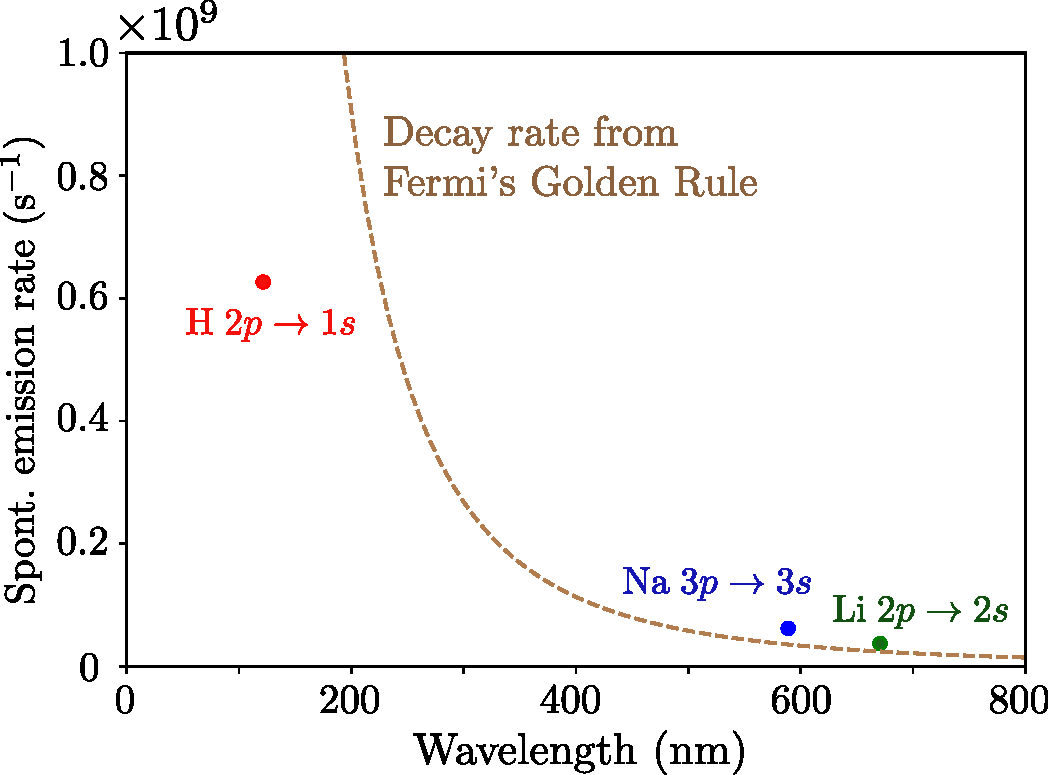
\includegraphics[width=0.6\textwidth]{emissionrates}
  \caption{Spontaneous emission rates (Einstein $A$ coefficients) for
    the $2p\rightarrow 1s$ transition in hydrogen, the
    $2p\rightarrow2s$ transition in lithium, and the $3p\rightarrow3s$
    transition in sodium.  Data points extracted from the NIST Atomic
    Spectra Database
    (\href{https://www.nist.gov/pml/atomic-spectra-database}{https://www.nist.gov/pml/atomic-spectra-database}).
    The dashed curve shows the decay rate based on Fermi's Golden
    Rule, with $|\mathbf{d}| \approx 10^{-10}\,\mathrm{m}$.  }
\end{figure}

%% Need to treat both electrons and photons on the same footing, with QFT
%% language.  Renormalization.

%% \section*{Exercises}

%% \begin{enumerate}
%% \item Gauge transformations.
%% \end{enumerate}

\section*{Further Reading}

\begin{enumerate}[[1{]}]
\item F.~J.~Dyson, \textit{1951 Lectures on Advanced Quantum Mechanics
  Second Edition}, arxiv:quant-ph/0608140. [\href{https://arxiv.org/abs/quant-ph/0608140}{link}]
\label{cite:dyson}

\item A.~Zee, \textit{Quantum Field Theory in a Nutshell} (Princeton
  University Press, 2010).
\label{cite:zee}

\item L.~L.~Foldy and S.~A.~Wouthuysen, \textit{On the Dirac Theory of
  Spin $1/2$ Particles and Its Non-Relativistic Limit}, Physical
  Review \textbf{78}, 29 (1950). [\href{https://journals.aps.org/pr/abstract/10.1103/PhysRev.78.29}{link}]
\label{cite:foldy}
\end{enumerate}

\end{document}


%% For decades after the discovery of quantum mechanics, the quantum
%% double-slit experiment was just a ``thought experiment'', meant to
%% illustrate the features of quantum mechanics that had been uncovered
%% by other, more complicated experiments.  Nowadays, the most convenient
%% way to do the experiment is with light, using single-photon sources
%% and single-photon detectors.  Quantum interference has also been
%% demonstrated experimentally using electrons, neutrons, and even
%% large-scale particles such as buckyballs.
